\documentclass[a4paper]{report}

%uncomment to see the references
%\usepackage{showkeys}
\usepackage[T2A]{fontenc}

\usepackage[section]{algorithm} % ???
\usepackage{algorithmic} % ???
\usepackage[english,russian]{babel}

\usepackage[backend=biber,bibencoding=utf8,sorting=none,sortcites=true,bibstyle=sty/gost71,maxnames=99,citestyle=numeric-comp,babel=other]{biblatex
}

\defbibenvironment{bibliography}
  {\list
     {\printfield[labelnumberwidth]{labelnumber}.}
     {\setlength{\labelwidth}{2\labelnumberwidth}%
      \setlength{\leftmargin}{\labelwidth}%
      \setlength{\labelsep}{\biblabelsep}%
      \addtolength{\leftmargin}{\labelsep}%
      \setlength{\itemsep}{\bibitemsep}%
      \setlength{\parsep}{\bibparsep}}%
      \renewcommand*{\makelabel}[1]{\hss##1}}
  {\endlist}
  {\item}


\usepackage[utf8]{inputenc}
\usepackage{csquotes} % ????
%\usepackage{expdlist}
%\usepackage[nottoc,notbib]{tocbibind}
\usepackage[pdftex]{graphicx}
\graphicspath{{pic/}}
\usepackage{tikz}


\usepackage{mathtools} % xmapsto, \Vector

\usepackage{comment}
\usepackage[colorinlistoftodos,prependcaption]{todonotes} % TODO: move to preamble!!
\presetkeys%
    {todonotes}%
    {inline,backgroundcolor=red}{}
\newcommand{\mtodo}[1]{\todo[linecolor=green!70!white, backgroundcolor=blue!20!white, bordercolor=red]{#1}}


\usepackage{soul} % text striking
\usepackage{amsmath,amsfonts,amssymb,amsthm,amscd,amsxtra}
\usepackage{physics}
\usepackage[sharp]{easylist}
\usepackage{siunitx}
\usepackage{sty/kbordermatrix}
\sisetup{locale=US}


\usepackage{sty/dbl12}
%\usepackage{srcltx}
\usepackage{epsfig}
% \usepackage{verbatim}
\usepackage{sty/rac}
\usepackage[singlelinecheck=false,font=large,labelfont=bf]{caption}

\usepackage{xcolor, colortbl}

% to generate index http://tex.stackexchange.com/a/42345/5966
\usepackage{hyperref}
\hypersetup{pdftex,colorlinks=true,allcolors=blue}
\usepackage{hypcap}
% 


\definecolor{light-gray}{RGB}{230,230,230}
\definecolor{dkgreen}{RGB}{0,154,0}
\definecolor{gray}{RGB}{128,128,128}
\definecolor{mauve}{RGB}{149,0,210}
\definecolor{purpur}{RGB}{255,204,153}
%%%%%%%%%%%%%%%%%%%%%%%%%%%%%%%%%%%%%%%%%%%%%%%%%%%%%%%%%%%%%%%%%%%%%%%%%%%%%%

\captionsetup[figure]{justification=centering,   position=bottom, skip=0pt}
\captionsetup[table] {justification=raggedright, position=top,    skip=0pt}

% Redefine margins and other page formatting

\setlength{\oddsidemargin}{0.5in}

% Various theorem environments. All of the following have the same numbering
% system as theorem.

\theoremstyle{plain}
\newtheorem{theorem}{Теорема}
\newtheorem{prop}[theorem]{Утверждение}
\newtheorem{corollary}[theorem]{Следствие}
\newtheorem{lemma}[theorem]{Лемма}
\newtheorem{question}[theorem]{Вопрос}
\newtheorem{conjecture}[theorem]{Гипотеза}
\newtheorem{assumption}[theorem]{Предположение}

\theoremstyle{definition}
\newtheorem{definition}[theorem]{Определение}
\newtheorem{notation}[theorem]{Обозначение}
\newtheorem{condition}[theorem]{Условие}
\newtheorem{example}[theorem]{Пример}
%\newtheorem{algorithm}[theorem]{Алгоритм}
\floatname{algorithm}{Листинг}
\renewcommand{\algorithmicrequire}{\textbf{Вход:}}

\renewcommand{\proofname}{Доказательство}

%\newtheorem{introduction}[theorem]{Introduction}

\renewcommand{\proof}{\\\textbf{Доказательство.}~}
 
\newcommand{\hilb}[1]{\mathcal{H}_{#1}}
\newcommand{\cconj}[1]{\overline{#1}}
\newcommand{\hank}[1]{H_{#1}^{(1)}}

\newcommand{\mcF}{\mathcal{F}}
\newcommand{\mcH}{\mathcal{H}} % ???
\newcommand{\mcI}{\mathcal{I}}
\newcommand{\mcL}{\mathcal{L}} % L2 space
\newcommand{\mcO}{\mathcal{O}} % Big O
\newcommand{\mcP}{\mathcal{P}}


\newcommand{\bbC}{\mathbb{C}} % complex plane
\newcommand{\bbD}{\mathbb{D}} % complex unit disk
\newcommand{\bbH}{\mathbb{H}} % complex upper half-plane TODO add to template
\newcommand{\bbN}{\mathbb{N}}
\newcommand{\bbK}{\mathbb{K}}
\newcommand{\bbR}{\mathbb{R}}
\newcommand{\bbT}{\mathbb{T}} % complex unit circle
\newcommand{\bbZ}{\mathbb{Z}}

\newcommand{\eqdef}{\overset{\mathrm{def}}{=\joinrel=}}

\DeclareMathOperator{\dom}{dom}
\DeclareMathOperator{\ran}{Ran}
\DeclareMathOperator{\rng}{rng}

\newcommand{\todo}[1]{\textcolor{red}{{\large TODO: #1}}}

\newenvironment{elist}{\begin{easylist}[enumerate]}{\end{easylist}}
\newenvironment{ilist}{\begin{easylist}[itemize]}{\end{easylist}}

\newcommand{\myspecial}[1]{\mathrm{#1}}

% imaginary unit
\newcommand{\iu}{{i\mkern1mu}}


\newcommand{\ipcdot}{\ip{\cdot}{\cdot}}
\newcommand{\iip}[2]{[#1,#2]}
\newcommand{\iipcdot}{\iip{\cdot}{\cdot}}

\newcommand{\dsum}{\oplus}
\newcommand{\ddiff}{\ominus}
% indefinite direct sum
\newcommand{\idsum}{[+]}
\newcommand{\iddiff}{[-]}

\DeclarePairedDelimiter{\Vector}{\lparen}{\rparen}

\newcommand{\tit}{\textit}
\newcommand{\cls}{\overline}
\newcommand{\eps}{\varepsilon}


\newcommand{\argmin}{\operatornamewithlimits{argmin}}
\newcommand{\argmax}{\operatornamewithlimits{argmax}}

\renewcommand{\Re}{\operatorname{Re}}
\renewcommand{\Im}{\operatorname{Im}}
\renewcommand{\phi}{\varphi} % TODO is there a prettier way to do that

\newcommand{\eexp}[1]{e^{#1}}

\DeclareMathOperator\atanh{atanh}

% ???
% \newcommand{\abs}[1]{\left| #1 \right|}
% \newcommand{\norm}[1]{\left\lVert #1 \right\rVert}
\newcommand*\Eval[3]{\left.#1\right\rvert_{#2}^{#3}}

% \lstnewenvironment{snippet}[1][]%
% {
%    \noindent
%    \minipage{\linewidth} 
%    \vspace{0.5\baselineskip}
%    \lstset{basicstyle=\ttfamily\footnotesize,frame=single,#1}}
% {\endminipage}

%\theoremstyle{remark}
%\newtheorem{remark}[theorem]{Remark}
%\include{header}
%%%%%%%%%%%%%%%%%%%%%%%%%%%%%%%%%%%%%%%%%%%%%%%%%%%%%%%%%%%%%%%%%%%%%%%%%%%%%%%

\numberwithin{theorem}{chapter}        % Numbers theorems "x.y" where x
                                        % is the section number, y is the
                                        % theorem number

%\renewcommand{\thetheorem}{\arabic{chapter}.\arabic{theorem}}

%\makeatletter                          % This sequence of commands will
%\let\c@equation\c@theorem              % incorporate equation numbering
%\makeatother                           % into the theorem numbering scheme

%\renewcommand{\theenumi}{(\roman{enumi})}

%%%%%%%%%%%%%%%%%%%%%%%%%%%%%%%%%%%%%%%%%%%%%%%%%%%%%%%%%%%%%%%%%%%%%%%%%%%%%%

\binoppenalty=10000
\relpenalty=10000

\addbibresource{thesis.bib}

\begin{document}
 % \renewcommand{\thelstlisting}{\thesection.\arabic{lstlisting}}
% Begin the front matter as required by Rackham dissertation guidelines
\initializefrontsections

\pagestyle{title}

\begin{center}
Университет ИТМО

\vspace{2cm}

Естественно-научный факультет

Кафедра высшей математики

\vspace{3cm}

{\Large Герасимов Дмитрий Александрович}

\vspace{2cm}

\vbox{\LARGE\bfseries
Исследование полноты резонансных состояний оператора Шредингера для модели квантовых графов
}

\vspace{4cm}

{\Large Научный руководитель: доктор физ.-мат. наук, \\ профессор кафедры ВМ И.~Ю.~Попов}

\vspace{6cm}

Санкт-Петербург\\ 2016
\end{center}

\newpage

\setcounter{page}{3}
\pagestyle{plain}

\tableofcontents
%\listoffigures

% Chapters
\startthechapters
\startprefacepage

Исследования резонансов и резонансных состояний различных физических систем проводились давно, начиная с классической работы лорда Рэлея \cite{rayleigh1916theory}, и по наши дни. Однако, строгое математическое обоснование и формализм этим являниям были даны во второй половине XX века. Теперь известно, что резонансы являются собственными числами, а резонансные состояние — собственными функциями некого диссипативного оператора \cite{lax1990scattering, adamjan1965class}.

Одним из интересных как с математической, так и физической точек зрения вопросов является вопрос о полноте резонансных состояний. Рассмотрим некий конечный резонатор $\Gamma$ с граничным условием Дирихле или Неймана. Как хорошо известно из теории операторов и рассеяния \cite{reed1980methods}, оператор Шредингера в такой области будет обладать чисто дискретным спектром и полной системой собственных функций в $\mcL^2(\Gamma)$. Теперь применим к резонатору возмущение, соединив его через небольшое отверстие с волноводом. После этого, у системы будет непрерывный спектр, а собственные значения исходной системы превращаются в резонансы и «смещаются» в комплексную плоскость. Резонансные состояния формально удовлетворяют уравнению Шредингера и граничным условиям, однако не квадратично интерируемы, так как их волновые функции не уходят в ноль на бесконечности, то есть не являются собственными функциями оператора Шредингера на новом домене. Однако, при сужении этих резонасных состояний на конечный домен $\Omega$, они вновь становятся интегрируемыми и принадлежат простанству $\mcL_2(\Omega)$. Интересным является вопрос о полноте этих суженных состояний на домене $\Omega$, и соответственно, вопрос о поиске такого поддомена квантовой системы, на котором его резонансные состояния будут полны. Существует гипотеза о том, что таким поддоменом является выпуклая оболочка рассеивателя. \todo{сослаться на работы которые уже были?}

% Квантовый граф — широко используемая модель наносистемы \cite{kuchment2002graph, lobanov2013genetic, 3, 4}. Если граф $\Gamma$ состоит только из конечного числа ребер конечной длины, его гамильтониан имеет чисто дискретный спектр, и его собственные функции образуют полную систему в $\mcL_2(\Gamma)$. Если же граф $\Gamma$ представляет из себя резонатор $\Omega$ с полубесконечными ребрами, в спектре будет присутствовать непрерывная часть и резонансы, индуцированные собственными числами гамильтониана резонатора $\mcH_\Omega$. Резонансные состояния оператора Шредингера не принадлежат пространству $\mcL_2(\Gamma)$, однако, при сужении их на конечный домен $\Omega$, становятся квадратично интегрируемыми и лежат в пространстве $\mcL_2(\Omega)$. Для многих приложений интересно знать, формируют ли полную систему резонанстные состояния графа $\Gamma$ в пространстве $\mcL_2(\Omega)$ резонатора.

В статье \cite{popov_exner70} была показана полнота резонансных функций на графе с резонатором, состоящим из отрезка, связанным с волноводом $\delta$-образным барьером. Естественным предположением является что произвольный резонатор состоящий из конечного числа ребер конечной длины должен обладать похожими свойствами, однако, мы покажем, что это не так. 

Целью данной работы является исследование нескольких моделей квантовых графов и анализ их резонансных состояний на предмет их полноты на области резонатора.
\chapter{Предварительные сведения}
\label{chapter1}

\section{Уравнение Шредингера}
\todo{рассеиватель}

\todo{резонаторы}

\section{S-матрица}

\todo{картиночку с полюсами и нулями??}

В общем виде волновые функции, являющиеся решениями уравнения Шредингера слева и справа от резонатора имеют вид:
\[
\psi_L(x) = A \eexp{\iu k x} + B \eexp{-\iu k x}
\]
\[
\psi_R(x) = C \eexp{\iu k x} + D \eexp{-\iu k x}
\]

S-матрица (матрица рассеяния) выражает зависимость исходящей волны от входящей:
\[
\begin{pmatrix} B \\ C \end{pmatrix} = S \begin{pmatrix} A \\ D \end{pmatrix}
\]

\todo{свойства}

\todo{симметричный/несимметричный случай}

\section{Преобразование Кэли}

Прямое преобразование Кэли (англ. Cayley transform) конформно отображает верхнюю комплексную полуплоскость (англ. upper half-plane) $\bbH = \{ x + \iu y \mid y > 0, x, y \in \bbR \}$ в комплексный единичный круг (англ. unit disk) $\bbD = \{ z \mid \abs{z} < 1 \}$:
\begin{equation}\label{eq:cayley}
W(z) = \frac{z - \iu}{z + \iu}
\end{equation}
, обратное преобразование Кэли аналогично отображает $\bbD$ в $\bbH$:
\[
w(\zeta) = \iu \frac{1 + \zeta}{1 - \zeta}
\]

Важным свойством преобразование Кэли является инъективное отображение $\bbR$ в единичную окружность $\bbT = \partial \bbD =  \{z \mid \abs{z} = 1 \}$

\todo{перенести то что дальше куда-нибудь?}
Так как преобразование Кэли является трансформацией Мебиуса, оно сохраняет окружности. В частности, окружность с радиусом $r$ в нуле, под действием обратного преобразование Кэли перейдет в окружность с центром $C(r)$ и радиусом $R(r)$, где:

\begin{equation}
\begin{aligned}
   C(r) &= \Im \frac{w(r) + w(-r)}{2}
\\ R(r) &= \Im \frac{w(r) - w(-r)}{2}
\end{aligned}
\end{equation}

Легко заметить, что при стремлении $r$ к $1$, $R(r)$ стремится к бесконечности, а $C(r)$ стремится к $R(r)$, что естественно так как в пределе комплексная единичная окнужность отображается в вещественную ось.

\todo{написать про нотацию $z$ vs $\zeta$}

\todo{нотация, может сделать секцию?}

\todo{использовать шаблоны определений, теоремы и т.п.}

\section{Внутренние функции и произведение Бляшке}
Для скалярных внутренних функций $\phi$ определенных на комплексном единичном диске $\bbD$, существует критерий отстутствия сингулярного множителя \cite[стр. 99]{nikolskii}:
\[
\lim\limits_{r = 1} \int\limits_{\bbT} \log \abs{\phi(r \zeta)} d m(\zeta) = 0
\]

Так как $\det S$ является скалярной внутренней функцией, мы можем воспользоваться данным критерием для исследования полноты системы резонантных состояний.

\todo{мутно}

\todo{Неравенство Коши-Шварца??}

\section{Фиксирование нотации}
\subsection{Различные обозначения}

\begin{ilist}
# Жирным обозначаются вектора: к примеру, $\vb{r} \in \bbR^n$, без выделения жирным — их длины: $r = |\vb{r}|$;
# Сопряжение комплексных чисел обозначается как $\cconj{c}$;
# Сопряжение операторов обозначается как $A^*$.
\end{ilist}

\subsection{Скалярное произведение}

В данной работе используется \textbf{физическая} нотация. В частности, это означает, что скалярное произведение в $L^2(E)$ определено как $\ip{f}{g} = \int\limits_E \cconj{f(\vb{x})} g(\vb{x}) \dd \vb{x}$.

\section{Терминология теории рассеяния}
Состояния рассеяния (англ. scattering states) — решения уравнения Шредингера, соответствующие непрерывному спектру, и не лежащие в $L^2$. Также частно называется каналом рассеяния (англ. scattering channel).

Мода (англ. mode) — связанная часть состояния рассеяния. О них обычно говорят в контексте волноводов, имеющих двумерную или трехмерную геометрию, и допускающих только связанные состояния в поперечном направлении. К примеру, в волноводе с конфигурацией $\Omega = [-\infty, \infty] \times [0, H]$ допустимыми поперечными модами являются $\psi_n(y) = \sqrt{\frac{2}{H}} \sin(\frac{\pi n}{H} y)$, $n \in \bbN^+$. Если поперечной частью волны является мода $n$, говорят, что «волна распространяется на $n$-й моде».

Открытый канал (англ. open channel) — канал рассеяния, на котором волна потенциально может распространяться при данной энергии $E$. Закрытый канал (англ. closed channel) — канал рассеяния, на котором волна не может распространяться при данной энергии $E$. Для вышеупомянутого примера двумерного волновода при любой энергии $E$ всегда будут открыты каналы $\{n \mid n \in \bbN^+, \left(\frac{\pi n}{H}\right)^2 < E \}$, которых, очевидно, конечное число. % TODO rename to 'survey'?
\chapter{Описание реализованного подхода}

\section{Модель резонатора типа «пучок»}\label{sec:bundle} % MINOR TODO пучок? =/

\todo{описание}

\todo{figure}

\todo{Определитель $S$-матрицы в замкнутой форме}


\newpage

\section{Модель резонатора типа «кольцо»}\label{sec:ring}
\subsection{Модель исследования}
% TODO http://tex.stackexchange.com/a/155317/5966 ?
\begin{figure}[!htb] % TODO maybe just ref instead?
\begin{tikzpicture}[scale=0.8] % TODO SCALE!!!
\newcommand{\Wglen}{6.0}; % waveguide length
\newcommand{\Warrlen}{2.0}; % wave arrow length
\newcommand{\Reslen}{0.0}; % resonator length

\coordinate (LLL) at (-\Wglen - 1, 0);
\coordinate (RRR) at ( \Wglen + 1, 0);
\coordinate (LL)  at (-\Wglen, 0);
\coordinate (RR)  at ( \Wglen, 0);
\coordinate (L)   at (-\Reslen, 0);
\coordinate (R)   at ( \Reslen, 0);
%

\coordinate (U) at (0, 3); % upper point of resonator

% waveguide
\draw[ultra thick, dotted] (LLL) -- (LL);
\draw[ultra thick] (LL)--(L);
\draw[ultra thick] (R)--(RR);
\draw[ultra thick, dotted] (RR) -- (RRR);
%

\draw[<-, thick] (-\Wglen, 1.5) -- (-\Wglen + \Warrlen, 1.5) node [midway, above] {\large $R e^{-\iu k x}$};
\draw[->, thick] (-\Wglen, 0.8) -- (-\Wglen + \Warrlen, 0.8) node [midway, above] {\large $e^{\iu k x}$};
\draw[->, thick] (\Wglen - \Warrlen, 0.5) -- (\Wglen, 0.5)   node [midway, above] {\large $T e^{\iu k x}$};

\draw (LL) node [below] {\large $\Omega_L$};
\draw (RR) node [below] {\large $\Omega_R$};

\draw[ultra thick] (0, 2) node [above] {\Large $\Omega$};

\draw[ultra thick] node [below] {\large $V$} (0, 2) circle[radius=2];
\end{tikzpicture}
\caption{квантовый граф $\Gamma$, состоящий из полубесконечных ребер $\Omega_L, \Omega_R$ и рассеивателя $\Omega$, представляющего из себя окружность длиной $1$.}
\end{figure}

Мы рассматриваем случай рассеяния волны c волновым вектором $k$, приходящей слева направо. Таким образом, волновые функции на различных частях графа принимают следующий вид:

\begin{equation}\label{eq:ring_system}
\begin{aligned}
\psi_L(x) &= \eexp{\iu k x} + R \eexp{-\iu k x} \\
\psi_R(x) &= T \eexp{\iu k x}\\
\psi_\Omega(x) &= P \sin(k x) + Q \cos(k x)
\end{aligned}
\end{equation}
, где $R$ и $T$ — коэффициенты отражения и прохождения волны. Так как граф симметричен, его матрица рассеяния принимает вид
$S(k) = \begin{pmatrix} R(k) & T(k) \\ T(k) & R(k) \end{pmatrix}$.

В вершине $V$ мы ставим $\delta$-образную потенциальную яму высотой $a$, которая порождает следущие граничные условия:

\begin{equation}\label{eq:ring_bc}
\begin{aligned}
\psi_L(0) = \psi_R(0) = \psi_\Omega(0) = \psi_\Omega(1) \\ 
-\psi'_L(0) + \psi'_\Omega(0) - \psi'_\Omega(1) + \psi'_R(0) = a \psi_L(0)
\end{aligned}
\end{equation}


\subsection{Вычисление S-матрицы}
Определим коэффициенты прохождения и отражения, подставив функции (\ref{eq:ring_system}) в (\ref{eq:ring_bc}) и решив систему линейных уравнений:
\begin{align*}
& 1 + R &= T \\
& 1 + R &= Q \\
& Q \cos k + P \sin k &= T \\
& -P k \cos k + Q k \sin k + P k + \iu R k + \iu T k - \iu k &= T a
\end{align*}

Решив систему, получаем:

\begin{align*}
R(k) = -\frac{2 \, k \cos\left(k\right) + a \sin\left(k\right) - 2 \, k}{2 \, k \cos\left(k\right) + {\left(a - 2 i \, k\right)} \sin\left(k\right) - 2 \, k} \\
T(k) = -\frac{2 i \, k \sin\left(k\right)}{2 \, k \cos\left(k\right) + {\left(a - 2 i \, k\right)} \sin\left(k\right) - 2 \, k}
\end{align*}
, подставляя полученные значения коэффициента прохождения и отражения в S-матрицу, получаем определитель S-матрицы в замкнутой форме:

\begin{equation}\label{eq:ring_detS}
\det S = 
\frac
{\cos\left(k\right) + {\left(\frac{a}{2 k} + i\right)} \sin\left(k\right) - 1}
{\cos\left(k\right) + {\left(\frac{a}{2 k} - i\right)} \sin\left(k\right) - 1}
\end{equation}


\subsection{Исследование полноты при $a=0$}
Рассмотрим случай $a=0$:
\[
\det S
= \frac
{\cos\left(k\right) + \iu \sin\left(k\right) - 1}
{\cos\left(k\right) - \iu \sin\left(k\right) - 1}
= \frac{\eexp{\iu k} - 1}{\eexp{-\iu k} - 1}
= -\eexp{i k}
\]

Из выражения выше легко заметить, что подынтегриальное выражение в (\todo{ссылку}) сводится к $\ln \abs{\det S} = \ln \eexp{- \Im k} = -\Im k$. Вычислим интеграл в пространстве единичного диска, для этого применим обратное преобразование Кэли $w(\zeta) = \iu \frac{1 + \zeta}{1 - \zeta}$, к подынтегральной функции: $\Im k \to \Im \left( \iu \frac{1 + \zeta}{1 - \zeta} \right) $.

\[
  \lim\limits_{R = 1} \int\limits_{\abs{\zeta} = R} \ln \abs{\det S(\zeta)} d \zeta
= \lim\limits_{R = 1} \int\limits_{\abs{\zeta} = R} \Im \left( \iu \frac{1 + \zeta}{1 - \zeta} \right)  d\zeta = \dots
\]
, параметризуем контур интегрирования полярными координатами: $\zeta \to R \eexp{\iu \phi}, d\zeta \to R \iu \eexp{\iu \phi}$:
\[
\dots = \lim\limits_{R = 1} \int\limits_{\abs{\zeta} = R} \Im \left( \iu \frac{1 + R \eexp{\iu \phi}}{1 - R \eexp{\iu \phi}} \right) R \iu \eexp{\iu \phi} d\phi
\]

Комплексный интеграл складывается из сумм интегралов действительной и мнимной части подынтегрального выражения. Рассчитаем мнимую часть:

\begin{align*}
   \Im \left(  \Im \left( \iu \frac{1 + R \eexp{\iu \phi}}{1 - R \eexp{\iu \phi}} \right) R \iu \eexp{\iu \phi} \right)
\\ &= R \Re \left(  \Re \left( \frac{1 + R \eexp{\iu \phi}}{1 - R \eexp{\iu \phi}} \right) \eexp{\iu \phi} \right)
\\ &= R \Re \left( \frac{1 + R \eexp{\iu \phi}}{1 - R \eexp{\iu \phi}} \right) \Re \left(   \eexp{\iu \phi} \right)
\\ &= R \Re \left( \frac{(1 + R \eexp{\iu \phi}) (1 - R \eexp{-\iu \phi}) }{(1 - R \eexp{\iu \phi}) (1 - R \eexp{-\iu \phi})} \right) \cos \phi
\\ &= R \Re \left( \frac{1 - R^2 + 2 \iu R \sin \phi}{1 + R^2 - 2 R \cos \phi} \right) \cos \phi
\\ &= R \frac{1 - R^2}{1 + R^2 - 2 R \cos \phi} \cos \phi 
% \\ &= \frac{1 - R^2}{2} \frac{\cos \phi}{\frac{1 + R^2}{2R} - \cos \phi} 
\end{align*}

\todo{доинтегрировать}

Интегрируя, получаем $2 \pi R^2$, что значит, что предел мнимой части при $R \to 1$ равен $2 \pi$, следовательно, по критерию полноты, система резонатных состояний графа $\Gamma$ не является полной на кольце $\Omega$.

\todo{график S-матрицы?}


\subsection{Исследование полноты при $a \ne 0$}
\todo{опровергнуть!!}

\todo{Объяснить результат}

\todo{другие виды резонаторов?}

\newpage

\section{Модель резонатора типа «решетка»}

\todo{????, показать результаты численного интегрирования? Не успею, наверное, аналитически. Можно хотя бы S-матрицу и помахать руками?} % TODO rename to 'description'?
\chapter{Результаты} 
\label{chapter3}

\todo{интерпретация результата?}

\todo{REWRITE}

Зафиксируем следующую геометрию волновода:
\begin{ilist}
# $L_x = 200$ боровских радиусов (порядка 10 нм);
# $L_y = 100$ боровских радиусов (порядка 5 нм);
# $H = 100$ боровских радиусов (порядка 5 нм);
# $S = 10$ боровских радиусов (порядка 0.5 нм).
\end{ilist}
Пусть слева поступает входящая волна на первой моде:
\[
\psi_{inc}(x, y) = \sqrt{\frac{2}{H}} \sin(\frac{\pi}{H} y) e^{i \sqrt{E - \pi^2 / H^2}}
\]
Далее приведены результаты, полученные в рамках подхода, описанного в главе 2.
\section{Зависимость коэффициента прохождения от энергии входящей волны при фиксированной геометрии резонатора}
% \begin{figure}[H]
% 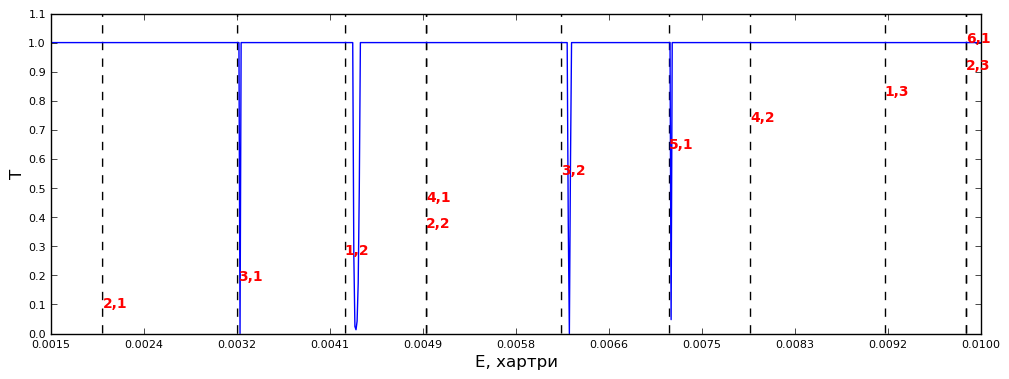
\includegraphics[width=1.0\textwidth]{transmission_all.png}
% \caption{Зависимость коэффициента прохождения от энергии при фиксированной геометрии. Вертикальные пунктирные линии соответствуют собственным энергиям резонатора, красными парами чисел обозначены номера состояний.}
% \label{fig:transmission_all}
% \end{figure}
% Как и ожидалось, в большинстве случаев коэффициент прохождения равен $1$. Падения коэффициента прохождения соответствуют тому, что волновая функция «чувствует» резонатор при некоторых энергиях, имеющих некоторую связь с собственными энергиями резонатора.

\section{Плотности вероятности}
% \begin{figure}[H]
% 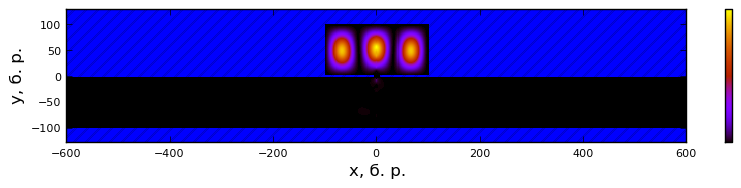
\includegraphics[width=1.0\textwidth]{pdensity_31_r.png}
% \caption{Плотность вероятности в резонансной точке.}
% \label{fig:pdensity_31_r}
% \end{figure}
% На рисунке~\ref{fig:pdensity_31_r} можно наблюдать плотность вероятности волновой функции в точке, соответствующей  резонансу на рисунке~\ref{fig:transmission_31}. Как и ожидалось, она вся сконцентрирована в области резонатора, и потока вероятности через волновод почти не наблюдается, коэффициент прохождения равен $0$.

\section{Зависимость коэффициента прохождения от геометрии резонатора} % TODO rename to 'results'?
\startconclusionpage

В работе исследовано поведение системы резонансных состояний различных квантовых графов, в частности, аналитически исследован вопрос полноты. Резонансные состояния таких систем сложно получить в явном виде, и соответственно, доказать полноту системы напрямую. Данная работа отличается новизной, так как ранее подобное исследование было проведено только для двух простейших моделей резонаторов \cite{spectralpavlov16}.

В \autoref{sec:bundle} была доказана полнота резонансных состояний для квантового графа сложной формы. Выработанный подход к доказательству может быть обобщен и использован для доказательства полноты для других граничных условий и квантовых графов.

В \autoref{sec:ring} было показано качественно различное поведение, казалось бы, похожих моделей и показано что полнота системы может быть потеряна в ходе непрерывной трансформации квантового графа и его граничных условий. Это является весьма важным свойством, которое означает что исследование полноты системы резонансных состояний сложного квантового графа не всегда может быть легко сведено к исследованию полноты для более простого квантового графа, полученного, например, стягиванием ребер исходного, и возможно, для исследования полноты произвольного квантового графа необходим некий сложный шаг индукции, если не другой подход. Также заметим, что в произвольном квантовом графе ребра могут соединять либо две разные вершины, либо быть петлей, что и является резонатором типа «кольцо», исследованным в данной работе. 

Проведенное исследование является важной подзадачей в более общей задаче нахождения пространства, в котором резонансные состояния квантового графа будут образовывать полную систему.

Естественным продолжением данной работы может являться исследование полноты системы резонансных состояний при других граничных условиях в точке соединения резонатора и волновода.
% \chapter{Trash}
\label{trash}

\subsection{Дефектные элементы}
Пусть направление нормали к границе между областями совпадает с осью $y$, тогда: дефектный элемент

\subsection{Волновод}



\subsection{Цилиндрические координаты}

\[
\vb{r} = (r, \theta, z)
\]


\subsection{Волновод}


\subsection{Преобразование Фурье}
В задачах квантовой механики часто удобно и более естественно производить анализ в импульсном представлении, нежели чем в координатном. Они связаны между собой преобразованием Фурье (напоминаем, что пользуемся АСЕ, засчет чего константа $\hbar$ опускается):

\subsubsection{Из координатного представления в моментное}
Пусть имеется волновая функция $\psi: \bbR^n \to \bbC$. 

\subsubsection{Из импульсного представления в координатное}


\printbibliography

\newpage
\listoftodos[Notes]

%\startappendices
%\input{parts/appendix1.tex}

\end{document}
